% ----------------------------------------------------
% PR Integration
% ----------------------------------------------------
\documentclass[class=report,11pt,crop=false]{standalone}
% Page geometry
\usepackage[a4paper,margin=20mm,top=25mm,bottom=25mm]{geometry}

% Font choice
\usepackage{lmodern}

% Use IEEE bibliography style
\bibliographystyle{IEEEtran}

% Line spacing
\usepackage{setspace}
\setstretch{1.20}

% Ensure UTF8 encoding
\usepackage[utf8]{inputenc}

% Language standard (not too important)
\usepackage[english]{babel}

% Skip a line in between paragraphs
\usepackage{parskip}

% For the creation of dummy text
\usepackage{blindtext}

% Math
\usepackage{amsmath}

% Header & Footer stuff
\usepackage{fancyhdr}
\pagestyle{fancy}
\fancyhead{}
\fancyhead[R]{\nouppercase{\rightmark}}
\fancyfoot{}
\fancyfoot[C]{\thepage}
\renewcommand{\headrulewidth}{0.0pt}
\renewcommand{\footrulewidth}{0.0pt}
\setlength{\headheight}{13.6pt}

% Epigraphs
\usepackage{epigraph}
\setlength\epigraphrule{0pt}
\setlength{\epigraphwidth}{0.65\textwidth}

% Colour
\usepackage{color}
\usepackage[usenames,dvipsnames]{xcolor}

% Hyperlinks & References
\usepackage{hyperref}
\definecolor{linkColour}{RGB}{77,71,179}
\hypersetup{
    colorlinks=true,
    linkcolor=linkColour,
    filecolor=linkColour,
    urlcolor=linkColour,
    citecolor=linkColour,
}
\urlstyle{same}

% Automatically correct front-side quotes
\usepackage[autostyle=false, style=ukenglish]{csquotes}
\MakeOuterQuote{"}

% Graphics
\usepackage{graphicx}
\graphicspath{{Images/}{../Images/}}
\usepackage{makecell}
\usepackage{transparent}

% SI units
\usepackage{siunitx}

% Microtype goodness
\usepackage{microtype}

% Listings
\usepackage[T1]{fontenc}
\usepackage{listings}
\usepackage[scaled=0.8]{DejaVuSansMono}

% Custom colours for listings
\definecolor{backgroundColour}{RGB}{250,250,250}
\definecolor{commentColour}{RGB}{73, 175, 102}
\definecolor{identifierColour}{RGB}{196, 19, 66}
\definecolor{stringColour}{RGB}{252, 156, 30}
\definecolor{keywordColour}{RGB}{50, 38, 224}
\definecolor{lineNumbersColour}{RGB}{127,127,127}
\lstset{
  language=Matlab,
  captionpos=b,
  aboveskip=15pt,belowskip=10pt,
  backgroundcolor=\color{backgroundColour},
  basicstyle=\ttfamily,%\footnotesize,        % the size of the fonts that are used for the code
  breakatwhitespace=false,         % sets if automatic breaks should only happen at whitespace
  breaklines=true,                 % sets automatic line breaking
  postbreak=\mbox{\textcolor{red}{$\hookrightarrow$}\space},
  commentstyle=\color{commentColour},    % comment style
  identifierstyle=\color{identifierColour},
  stringstyle=\color{stringColour},
   keywordstyle=\color{keywordColour},       % keyword style
  %escapeinside={\%*}{*)},          % if you want to add LaTeX within your code
  extendedchars=true,              % lets you use non-ASCII characters; for 8-bits encodings only, does not work with UTF-8
  frame=single,	                   % adds a frame around the code
  keepspaces=true,                 % keeps spaces in text, useful for keeping indentation of code (possibly needs columns=flexible)
  morekeywords={*,...},            % if you want to add more keywords to the set
  numbers=left,                    % where to put the line-numbers; possible values are (none, left, right)
  numbersep=5pt,                   % how far the line-numbers are from the code
  numberstyle=\tiny\color{lineNumbersColour}, % the style that is used for the line-numbers
  rulecolor=\color{black},         % if not set, the frame-color may be changed on line-breaks within not-black text (e.g. comments (green here))
  showspaces=false,                % show spaces everywhere adding particular underscores; it overrides 'showstringspaces'
  showstringspaces=false,          % underline spaces within strings only
  showtabs=false,                  % show tabs within strings adding particular underscores
  stepnumber=1,                    % the step between two line-numbers. If it's 1, each line will be numbered
  tabsize=2,	                   % sets default tabsize to 2 spaces
  %title=\lstname                   % show the filename of files included with \lstinputlisting; also try caption instead of title
}

% Caption stuff
\usepackage[hypcap=true, justification=centering]{caption}
\usepackage{subcaption}

% Glossary package
% \usepackage[acronym]{glossaries}
\usepackage{glossaries-extra}
\setabbreviationstyle[acronym]{long-short}

% For Proofs & Theorems
\usepackage{amsthm}

% Maths symbols
\usepackage{amssymb}
\usepackage{mathrsfs}
\usepackage{mathtools}

% For algorithms
\usepackage[]{algorithm2e}

% Spacing stuff
\setlength{\abovecaptionskip}{5pt plus 3pt minus 2pt}
\setlength{\belowcaptionskip}{5pt plus 3pt minus 2pt}
\setlength{\textfloatsep}{10pt plus 3pt minus 2pt}
\setlength{\intextsep}{15pt plus 3pt minus 2pt}

% For aligning footnotes at bottom of page, instead of hugging text
\usepackage[bottom]{footmisc}

% Add LoF, Bib, etc. to ToC
\usepackage[nottoc]{tocbibind}

% SI
\usepackage{siunitx}

% For removing some whitespace in Chapter headings etc
\usepackage{etoolbox}
\makeatletter
\patchcmd{\@makechapterhead}{\vspace*{50\p@}}{\vspace*{-10pt}}{}{}%
\patchcmd{\@makeschapterhead}{\vspace*{50\p@}}{\vspace*{-10pt}}{}{}%
\makeatother
\makenoidxglossaries
% --------------------------------------------------------------------
% Examples of creating a glossary
\newacronym{cw}{CW}{Continuous-Wave}
\newacronym{dsp}{DSP}{Digital Signal Processing}
\newacronym{em}{EM}{Electromagnetic}
\newacronym{fmcw}{FMCW}{Frequency Modulated Continuous Wave}
\newacronym{gui}{GUI}{Graphical User Interface}
\newacronym{rf}{RF}{Radio Frequency}
\newacronym{radar}{RADAR}{Radio Detection and Ranging}
\newacronym{pcb}{PCB}{Printed Circuit Board}
\newacronym{pc}{PC}{Personal Computer}
\newacronym{pri}{PRI}{Pulse Repetition Interval}
\newacronym{adc}{ADC}{Analogue-to-Digital Converter}
\newacronym{if}{IF}{Intermediate Frequency}
\newacronym{itu}{ITU}{International Telecommunications Union}
\newacronym{rcs}{RCS}{Radar Cross Section}
\newacronym{opamp}{Op Amp}{Operational Amplifier}
\newacronym{gbwp}{GBWP}{Gain Bandwidth Product}
\newacronym{dc}{DC}{Direct Current}
\newacronym{ac}{AC}{Alternating Current}
\newacronym{uct}{UCT}{University of Cape Town}
\newacronym{usb}{USB}{Universal Serial Bus}
\newacronym{stft}{STFT}{Short-Time Fourier Transform}
\newacronym{fft}{FFT}{Fast Fourier Transform}
\newacronym{dft}{DFT}{Discrete Fourier Transform}
\newacronym{dtft}{DTFT}{Discrete-Time Fourier Transform}
\newacronym{snr}{SNR}{Signal-to-Noise Ratio}
\newacronym{prf}{PRF}{Pulse Repetition Frequency}
\newacronym{isar}{ISAR}{Inverse Synthetic Aperture}
% include SUV (check experimentation table)
% --------------------------------------------------------------------

\begin{document}
% ----------------------------------------------------
\chapter{Methodology \label{ch:methodology}}
\vspace{-1cm}
% ----------------------------------------------------
\section{Overview}
The focus of this study was to design an ultrasonic radar demonstrator to measure the speed of vehicles moving at speeds of at most 20 km/h in parking areas. This chapter aims to outline what research methods were used and the reasoning behind choosing these methods. A detailed explanation of the research process is provided to validate that the research was rigorously conducted and can therefore be accurately replicated. The approach to the research topic is explained, followed with an explanation of the system's operation. The tools and materials used to collect, validate, and analyse the data is presented in this chapter before sound justification is provided on the methodological choices made in the summary.

\section{Approach}
This study adopts a quantitative methodology as it consisted of collecting and analysing data. Furthermore, the methodology process was deductive as the research started off with established theory (explored in Chapter~\ref{ch:literature}) that was built on with the data collected through the research process. This quantitative approach was used to make predictions, test causal relationships, and find patterns in the results that could be used to make general statements that can be applied to similar ultrasonic radar systems. This methodology was chosen Due to the nature of the study, an Agile project management methodology was used, consisting of an iterative development process. This allowed regular tests, and effective changes, to be conducted to ensure the system operates in line with the requirements and specifications outlined at the start.

The research was largely experimental, as the results were conducted strictly in parking areas where cars are ideally moving at lower speeds than on the road. The demonstrator was designed to have variable parameters that could be manipulated to allow predictions to be made on the cause-and-effect between variables in the experiments. The vehicles in the experiment move in controlled environments where variables could not be manipulated. By conducting this research under a controlled environment, it allowed a causal relationship to be established between variables such as the speed of the vehicle and the bandwidth of the ultrasonic barrel transducers, or the distance between the demonstrator and its ability to detect a vehicle moving towards it.

An important consideration that was made, was the sampling strategy used. Specific vehicles were not selected for experimentation as this was thought to be impractical as it could place a time constraint on the project and make it challenging to find specific vehicle types in parking areas in the region. Because of this, data was collected from a random selection of cars that were found in parking areas in Rondebosch and Claremont in Cape Town. This ensured that data could be collected from motorcycles (due to the amount of deliveries that occur frequently in the area), buses (more specifically \gls{uct} \href{https://uct.ac.za/students/services-transport-parking-uct-shuttle/uct-shuttle-overview}{Jammie} shuttles), and an array of small to larger sized cars \footnote{Rondebosch is home to \gls{uct} which results in a number of student residences and accommodations being present in the area. Because of this, there is a good portion of small, budget cars driven by students including small-to-medium sized cars driven by an abundance of ride-hailing service drivers.}. The results were then analysed and discussed in Chapter~\ref{ch:results}.

%\section{System Operation}

\section{Data Collection and Validation}
Data was collected at various points in the project's life cycle - particularly for system testing and system implementation in the field. To test the system, lab equipment was used which included a handheld and desktop multimeter, an oscilloscope, a signal generator and a desktop power supply. These lab equipment were used to validate that the integrated system produced results similar to that generated through simulations. A \gls{usb} flash drive was used to collect voltage and frequency response data from the oscilloscope and is included in Chapter~\ref{ch:testing} of this report. Before the circuits were tested in a lab environment, they were simulated on \textsc{LTSpice XVII} which is a high performance \textsc{SPICE} simulator software for generating circuit schematics and producing simulations. The process used to collect data is illustrated in Figure~\ref{fig:data-collection}.

\begin{figure}[htbp]
    \centering
    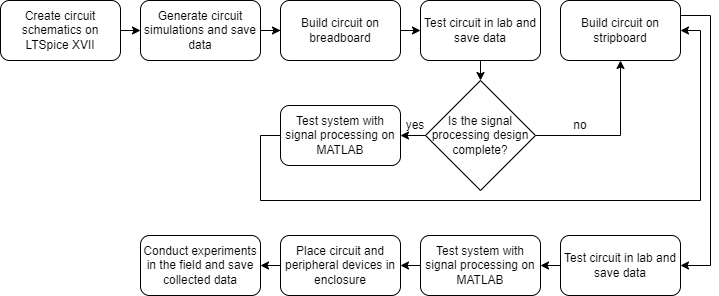
\includegraphics[width=0.8\columnwidth]{../Images/data_collection_methodology.drawio.png}
    \caption{Data collection approach}
    \label{fig:data-collection}
\end{figure}

Figure~\ref{fig:data-collection} shows the iterative testing process used to ensure accurate results were collected. The circuit was first built as schematics and simulated data was collected. Next, the circuit was built onto a breadboard and tested in the lab using the aforementioned lab equipment. Voltage outputs and frequency response results identical to that collected in the \textsc{LTSpice XVII} simulations were collected from the oscilloscope and the results were compared to validate the predictions from the simulations. In the case that the signal processing code was completed on \textsc{MATLAB}, this circuit was then integrated with the software and tested to ensure the system was producing accurate results. The circuit was then soldered onto a stripboard and tested in the lab again. This stripboard circuit was then loaded into an enclosure with the necessary peripheral devices (XONAR U5 sound card and 12 V power supply) and used to conduct experiments in the field. Furthermore, experiments were conducted in both indoor and outdoor parking areas to evaluate the relationship between the results provided and the demonstrator's performance.

\section{Data Analysis}
\textsc{MATLAB} and \textsc{LTSpice XVII} were used for data analysis in this study. \textsc{LTSpice XVII} was used to create schematics and generate various simulations to make predictions on the system's function before components could be ordered and it the system built.\textsc{MATLAB} was used to create the signal processing code required to determine the speed of the vehicles from the signals collected by the system. It was also used to create a user-friendly \gls{gui} that enabled data to be easily collected and analysed in the field. This software was used as they are free, easy to navigate and come equipped with available libraries and tools to accurately analyse the data collected at various points in the project's life cycle.

\section{Limitations}
With the key research design choices defined, the limitations of the design are explored. Given the constraints on the study, there have been trade-offs between the design and its practical implementation. A limitation to the project was having to create code in \textsc{MATLAB} that could accurately perform the signal processing tasks required for this study. To this effect, the thesis report provided by \cite{ian} and dissertation by \cite{clin} provided good groundwork for building the circuit \textit{and} the signal processing in \textsc{MATLAB}. Furthermore, the article written by \cite{asif} provides spectrogram results of extracted signatures a walking human using \textsc{MATLAB}. This report proved to be especially vital as an ultrasonic radar system and processed in \textsc{MATLAB}; this allowed the data collected when testing the circuit at various stages to be validated when tested in a similar fashion.

% Ideally, the circuit designs could have been re-evaluated to produce results that were more accurate with the calculations made in Chapter~\ref{ch:design}. Inaccurate practical results can have an effect on the results received during experiments. This limitation was reduced by continuously testing the circuit and providing slight adjustments to the components using components that were available in the lab at the time; any component change was adequately reported.

\section{Summary}
In summary, the study adopted a quantitative methodology approach with an Agile project management style to accommodate the amount of numerical data that was collected and analysed during the project and validate their accuracy. \textsc{LTSpice XVII} was used to analyse the system before implementation and \textsc{MATLAB} provided an accurate and reliable way for the data collected during experimentation to be validated and analysed. Overall, the methodology is thorough and rigorous, ensuring that the research is reliable and can be easily replicated.

% ----------------------------------------------------
\ifstandalone
\bibliography{../Bibliography/References.bib}
\printnoidxglossary[type=\acronymtype,nonumberlist]
\fi
\end{document}
% ----------------------------------------------------